\documentclass[conference]{IEEEtran}
\usepackage{graphicx}
\usepackage{booktabs}
\usepackage{amsmath}
\usepackage{url}
\usepackage[hidelinks]{hyperref}

\begin{document}

\title{When Fewer Bits Don't Save Energy: Measurement Pitfalls and a Negative Result for Precision Routing in LLM Inference}

% TODO: confirm with AI-SPC whether review is anonymous before filling in.
\author{\IEEEauthorblockN{Author One, Author Two, Author Three}
\IEEEauthorblockA{Sardar Patel Institute of Technology, Mumbai, India\\
\{author\}@spit.ac.in}}

\maketitle

\begin{abstract}
Weight quantization is widely assumed to reduce the energy of large language model (LLM) inference. We measure per-token GPU energy for Llama-3.2-1B at 4-bit (NF4), 8-bit (LLM.int8) and 16-bit (float16) using bitsandbytes at batch size~1, read from the GPU's on-board energy counter on an NVIDIA RTX~6000~Ada in a shared academic cluster. In three clean runs, 4-bit costs the same energy per token as float16 (1.6--1.7\,J/token) and 8-bit costs 1.8$\times$ more (3.1\,J/token): the quantized kernels draw less power but run 1.4--2.8$\times$ slower. Our main finding concerns measurement itself. On the shared node, the float16 measurement was inflated by up to 7.7$\times$ in daytime runs while the GPU was not shared and sat idle behind a slowed host-side launch path. An end-of-run co-tenancy check, agreement across repeated runs, and an automated validation gate all failed to detect this, and one previously accepted baseline was affected. Per-prompt throughput and power expose it immediately. Finally, a fuzzy-logic router that picks a precision tier per prompt is no more accurate than a random router with the same tier mix and uses 38--49\% more energy than always serving float16.
\end{abstract}

\begin{IEEEkeywords}
LLM inference, energy measurement, quantization, bitsandbytes, measurement methodology, precision routing
\end{IEEEkeywords}

\section{Introduction}
Quantizing an LLM's weights to 8 or 4 bits shrinks its memory footprint by 2--4$\times$, and it is natural to expect a matching energy saving. Whether that holds depends on how the low-precision arithmetic is executed. The most widely used drop-in path, bitsandbytes in Hugging Face Transformers, dequantizes weights to 16-bit on the fly, and prior benchmarking found that this can increase inference energy~\cite{poddar2025}.

We set out to build on the opposite premise: a router that sends each prompt to the cheapest precision tier of one resident model able to answer it. Measuring that premise on a shared GPU cluster led to three contributions:
\begin{enumerate}
\item \textbf{A measurement pitfall that standard safeguards miss (§\ref{sec:pitfall}).} The same float16 model on the same GPU consumed between 1.6 and 13.0\,J/token depending on when it ran, while the GPU itself sat idle. Three safeguards accepted the inflated measurement. Per-prompt throughput and power, already derivable from standard energy logs, separate clean from disrupted runs.
\item \textbf{Per-token energy of bitsandbytes tiers at batch size~1 (§\ref{sec:results}).} 4-bit NF4 breaks even with float16 and 8-bit costs 1.8$\times$ more, refining prior batched measurements~\cite{poddar2025} for single-request inference with a hardware counter.
\item \textbf{A negative result for per-prompt precision routing (§\ref{sec:routing}).} A fuzzy router is no more accurate than random at the same tier mix and costs 65--76\,J/request more than static float16. Routing can only save what the tiers themselves save.
\end{enumerate}

\section{Related Work}
\textbf{Energy of LLM inference.} Poddar et al.~\cite{poddar2025} find that bitsandbytes 8- and 4-bit quantization raises inference energy to almost 2$\times$ at equal batch size (A6000, batch sizes 8--256, software estimators); only larger batches made quantized models cheaper. TokenPowerBench~\cite{niu2026tokenpower} measures joules per token across models from 1B to 405B parameters, and Vellaisamy et al.~\cite{vellaisamy2026} decompose Llama-3.2-1B request energy on H100/H200. These works characterise what inference costs; none examines how measurements are corrupted on shared infrastructure, our main concern.
\textbf{Measurement and quantization.} Zeus~\cite{you2023zeus} and LLMCarbon~\cite{faiz2024llmcarbon} measure or model deep-learning energy and carbon. LLM.int8()~\cite{dettmers2022int8} and NF4~\cite{dettmers2023qlora}, the methods we measure, and GPTQ~\cite{frantar2023gptq} and AWQ~\cite{lin2024awq} target memory and accuracy.
\textbf{Routing.} RouteLLM~\cite{ong2024routellm} and FrugalGPT~\cite{chen2023frugalgpt} route or cascade between \emph{different} models; our router chooses among precision tiers of \emph{one} model, worthwhile only if lower precision is cheaper.

\section{Methodology}
\label{sec:method}
\textbf{Model and tiers.} Llama-3.2-1B~\cite{llama3} via bitsandbytes: 4-bit NF4 with double quantization and float16 compute; 8-bit LLM.int8(); 16-bit float16. Each tier carries a LoRA adapter (rank 16/8/4, on \texttt{q\_proj}, \texttt{v\_proj}); one tier is resident at a time, with 5 discarded warm-up generations.

\textbf{Hardware.} NVIDIA RTX~6000~Ada (48\,GB, driver 610.43.02) in a shared two-GPU SLURM node (dual AMD EPYC, 224 threads); jobs request one GPU and 8 cores, with thread pools pinned to them.

\textbf{Workload.} 500 deduplicated prompts (200 easy, 150 medium, 150 hard) from TriviaQA, Alpaca, GSM8K and CodeAlpaca; greedy decoding, 128 new tokens maximum, batch size~1, seed 42.

\textbf{Energy.} Energy per generation is the change in the GPU's cumulative on-board counter (NVML \texttt{nvmlDeviceGetTotalEnergyConsumption}, mJ resolution) across the generation, bracketed by \texttt{torch.cuda.synchronize()}. It is GPU-board energy only. We log per-prompt energy, tokens and latency, from which we derive throughput (tok/s) and mean power (W). Generations of 1--2 tokens often read 0\,J because the counter does not advance, so J/token is reported as the median over prompts with $\geq$16 generated tokens (371--469 per tier).

\textbf{Accuracy and validation.} Routing accuracy uses a reference-match proxy on our prompts (numeric match, normalised substring match, or token-F1 $\geq$ 0.5). Every run passes an automated validator checking grid completeness, positivity, plausibility and oracle consistency.

\section{Measurement Pitfall on a Shared Cluster}
\label{sec:pitfall}
Table~\ref{tab:tiers} lists every measurement of the same code and GPU. 4-bit and 8-bit reproduce closely throughout; 16-bit does not, ranging from 1.59 to 12.97\,J/token. Accuracy and every routing decision were identical across runs; only time and energy changed.

\begin{table}[t]
\caption{Per-tier medians (prompts with $\geq$16 tokens). 16-bit varies 8$\times$ across runs; 4- and 8-bit do not.}
\label{tab:tiers}
\centering\small
\setlength{\tabcolsep}{3.5pt}
\begin{tabular}{lccccc}
\toprule
 & \multicolumn{3}{c}{16-bit} & 4-bit & 8-bit \\
Run & tok/s & W & J/tok & J/tok & J/tok \\
\midrule
S1, 3 runs (day)$^\dagger$ & 10.5--11.8 & 85 & 7.2--7.8 & 1.33 & 3.00 \\
Run 4 (day) & 6.2 & 81 & 12.97 & 1.52 & 2.82 \\
Run 5 (night) & 80.7 & 136 & 1.69 & 1.71 & 3.12 \\
Run 6 (night) & 81.8 & 142 & 1.73 & 1.71 & 3.10 \\
Run 7 (night) & 81.5 & 130 & 1.59 & 1.66 & 3.06 \\
\bottomrule
\multicolumn{6}{l}{\footnotesize $^\dagger$Session~1 ran without LoRA adapters.}
\end{tabular}
\end{table}

\begin{figure}[t]
\centering
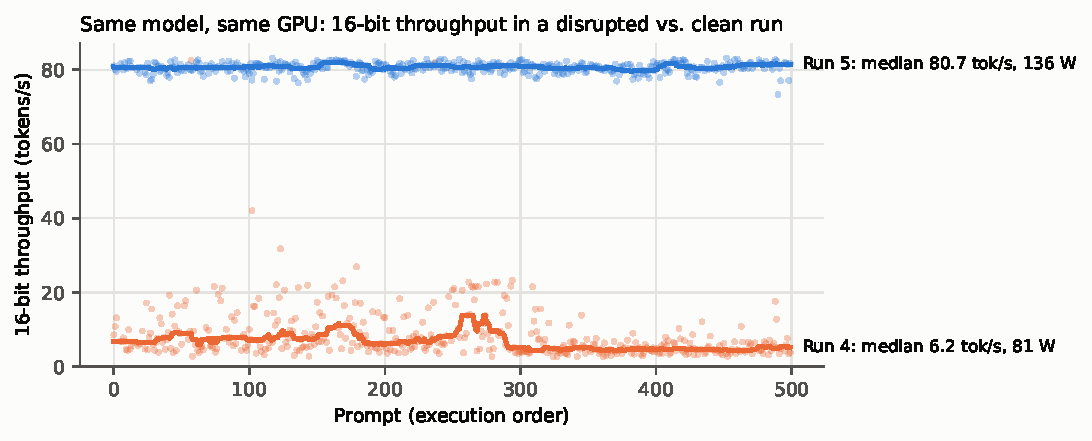
\includegraphics[width=\columnwidth]{figs/fig1_16bit_disruption.pdf}
\caption{16-bit throughput per prompt in a disrupted (run 4) and a clean (run 5) run of the same model on the same GPU. Lines: rolling median over 25 prompts.}
\label{fig:disruption}
\end{figure}

\textbf{The signature.} Clean 16-bit runs are fast \emph{and} power-hungry: about 81\,tok/s at 130--142\,W, steady to within $\pm$1\,tok/s across every tenth of the run (Fig.~\ref{fig:disruption}). Disrupted runs are slow \emph{and} low-power: 4--13\,tok/s at 81--85\,W, close to the GPU's mostly-idle draw. Since energy is power $\times$ time and a waiting GPU still draws substantial power, energy per token rises roughly in proportion to the slowdown.

\textbf{Host-side, not GPU-side.} The GPU was not shared. A diagnostic that times plain float16 generation, with no router, adapters or energy meter, ran in daytime at 8.5\,tok/s on average (4.4--25.6 over 12 repeats) with median GPU SM utilisation of 0\% and the process on-CPU 100\% of the time. The identical diagnostic at night ran at 109.9\,tok/s with a 1.01$\times$ spread: 13$\times$ faster on the same code and GPU. The GPU was waiting on a CPU-side launch path that had slowed by an order of magnitude; we did not isolate which shared host resource caused it. Disruption is not tier-specific: in an earlier run that interleaved tiers prompt by prompt under load, 16-bit was measured correctly and 4- and 8-bit were inflated 3--5$\times$. In by-tier runs, 16-bit ran last and coincided with the disruption.

\textbf{Why the safeguards missed it.} (1)~The co-tenancy snapshot is taken once, at the end of a run, and was empty for run~4 and for a run later confirmed contended. (2)~Session~1's three back-to-back runs agreed within 6.6\% and passed our pre-registered gate: agreement measured consistency, not cleanliness, and its 16-bit value has been withdrawn. (3)~The validator passed run~4, since its checks cannot see a uniform slowdown.

\textbf{Recommendation.} Report per-tier throughput and mean power alongside J/token; check throughput stability across the run (e.g.\ per-decile medians); re-measure any tier that departs from its clean baseline; record co-tenancy continuously, not once.

\section{Energy per Token by Precision}
\label{sec:results}
The three clean runs (5--7, on different nights; Table~\ref{tab:tiers}) give 1.66--1.71\,J/token for 4-bit, 3.06--3.12 for 8-bit and 1.59--1.73 for 16-bit. The 4-bit vs.\ 16-bit difference changes sign across runs ($+$1.4\%, $-$1.4\%, $+$4.4\%), so we report them as equal. Means over the same prompts agree with the medians, with 95\% CIs of $\pm$0.006 to $\pm$0.016\,J/token.

float16 draws the most power but is fastest; the quantized tiers draw less power but run 1.4$\times$ (4-bit) to 2.8$\times$ (8-bit) slower, and the extra time costs more energy than the lower power saves. Memory tells the opposite story: weights occupy 2.47\,GB in float16 (measured), and by calculation about 1.5\,GB at 8-bit and 1.0\,GB at 4-bit, because bitsandbytes leaves the 263\,M-parameter tied embedding in float16. Quantization here saves memory, not energy.

\section{Case Study: Per-Prompt Precision Routing}
\label{sec:routing}
\textbf{Router.} A sensor computes five features per prompt (Flesch--Kincaid grade, approximate token length, character entropy, dependency-parse depth, and a code/maths indicator), normalised to $[0,1]$ with ranges calibrated on the evaluation set. A Mamdani fuzzy controller (scikit-fuzzy; triangular low/medium/high memberships, seven rules, centroid defuzzification) maps them to a score in $[0,100]$, cut at 33/66 into 4-, 8- or 16-bit. Routing takes 10.1--10.3\,ms per prompt on the CPU, about 0.4\% of request latency.

\textbf{Baselines.} Static tiers; \emph{random-matched}, with exactly the router's tier mix (mean of 20 draws); \emph{threshold}, applying the same cuts to the plain feature mean; and an \emph{oracle} choosing, per prompt, the lowest-energy tier that answers correctly. Greedy decoding lets every condition be computed from one per-prompt $\times$ per-tier grid.

\begin{table}[t]
\caption{Routing results. Accuracy is identical in runs 5--7.}
\label{tab:routing}
\centering\small
\begin{tabular}{lcc}
\toprule
Condition & Accuracy & J/request (runs 5/6/7) \\
\midrule
Static 4-bit & 0.110 & 130 / 130 / 129 \\
Static 8-bit & 0.186 & 323 / 320 / 317 \\
Static 16-bit & 0.162 & 166 / 174 / 155 \\
Fuzzy router & 0.156 & 238 / 239 / 232 \\
Random, matched mix & 0.166 & 241 / 242 / 234 \\
Threshold & 0.120 & 185 / 184 / 182 \\
Oracle & 0.258 & 140 / 141 / 134 \\
\bottomrule
\end{tabular}
\end{table}

\begin{figure}[t]
\centering
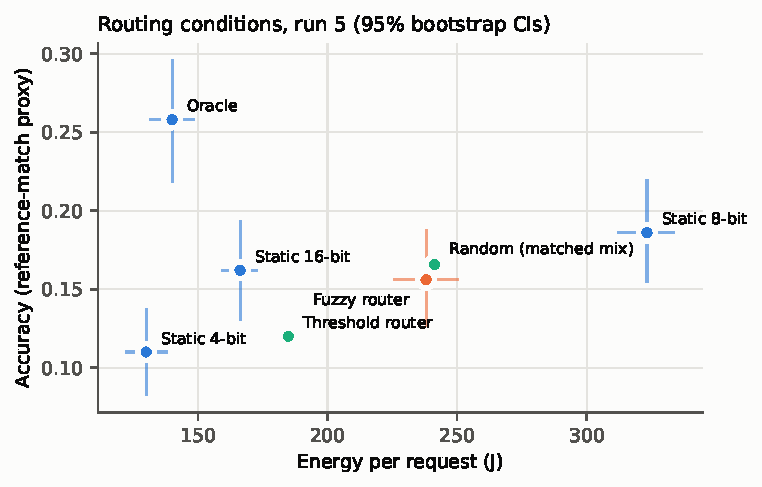
\includegraphics[width=0.92\columnwidth]{figs/fig3_routing_run5.pdf}
\caption{Accuracy vs.\ energy per request for each routing condition (run 5), with 95\% bootstrap CIs.}
\label{fig:routing}
\end{figure}

\textbf{Results.} Table~\ref{tab:routing} and Fig.~\ref{fig:routing}. A paired per-prompt bootstrap of fuzzy router minus static 16-bit gives $+$71.7 (95\% CI 61.0--82.2), $+$65.4 (54.9--75.8) and $+$76.4 (66.5--86.9)\,J/request in runs 5--7, i.e.\ 38--49\% more energy, with an accuracy difference of $-$0.006 (CI $-$0.034 to $+$0.020).

\textbf{Why it fails.} The sensor does respond to difficulty, sending 61\% of hard prompts to 16-bit against 21\% of easy ones, but it sends 52\% of all prompts to 8-bit, the most expensive tier. Its choice matches the oracle's on 27\% of prompts (run 5), below the 33\% of a uniform random pick. The oracle reaches 0.258 accuracy at 134--141\,J/request by using 4-bit where it suffices, float16 otherwise, and almost never 8-bit. Only 129 of 500 prompts are answered correctly by any tier under the proxy metric, which also caps what routing can gain.
% TODO Session 2: standard-benchmark accuracy per tier, with/without adapters (tinyBenchmarks), if job 1784 completes.

\section{Threats to Validity}
One model, one GPU and one library: kernels that compute natively in low precision (AWQ, FP8) and larger models may show real savings. Batch size~1 only; prior work finds quantized models cheaper at large batches~\cite{poddar2025}. GPU-board energy only, excluding CPU, DRAM and the router. The host mechanism behind the disruption is not isolated. The reference-match accuracy proxy is coarse; routing conclusions rest mainly on energy. All Session~4 tiers carry LoRA adapters.

\section{Conclusion}
Measured with a hardware counter at batch size~1, bitsandbytes 4-bit quantization of a 1B-parameter LLM saves memory but not energy, and 8-bit costs 1.8$\times$ more than float16. Getting this right was harder than expected: on a shared cluster, a host-side slowdown inflated float16 energy by up to 7.7$\times$, passed every safeguard we had, and contaminated a baseline. Reporting per-prompt throughput and power alongside energy catches it. A fuzzy per-prompt precision router, built on the assumption that fewer bits cost less, uses more energy than never quantizing. Future work will test whether native low-precision kernels and larger models change the picture, and whether routing becomes worthwhile when they do.

\bibliographystyle{IEEEtran}
\bibliography{refs}

\end{document}
